% Lorentz.tex      pdflatex ZhCvGo15
% Diffuse globally, compute locally: a cyclist tale
% Tingnan Zhang, Daniel I. Goldman and Predrag Cvitanovi\'c

%\section{Diffusion in periodic arrays}
%\label{s-DiffPerArr}

\begin{figure}[htbp]
  \begin{center}
    (a)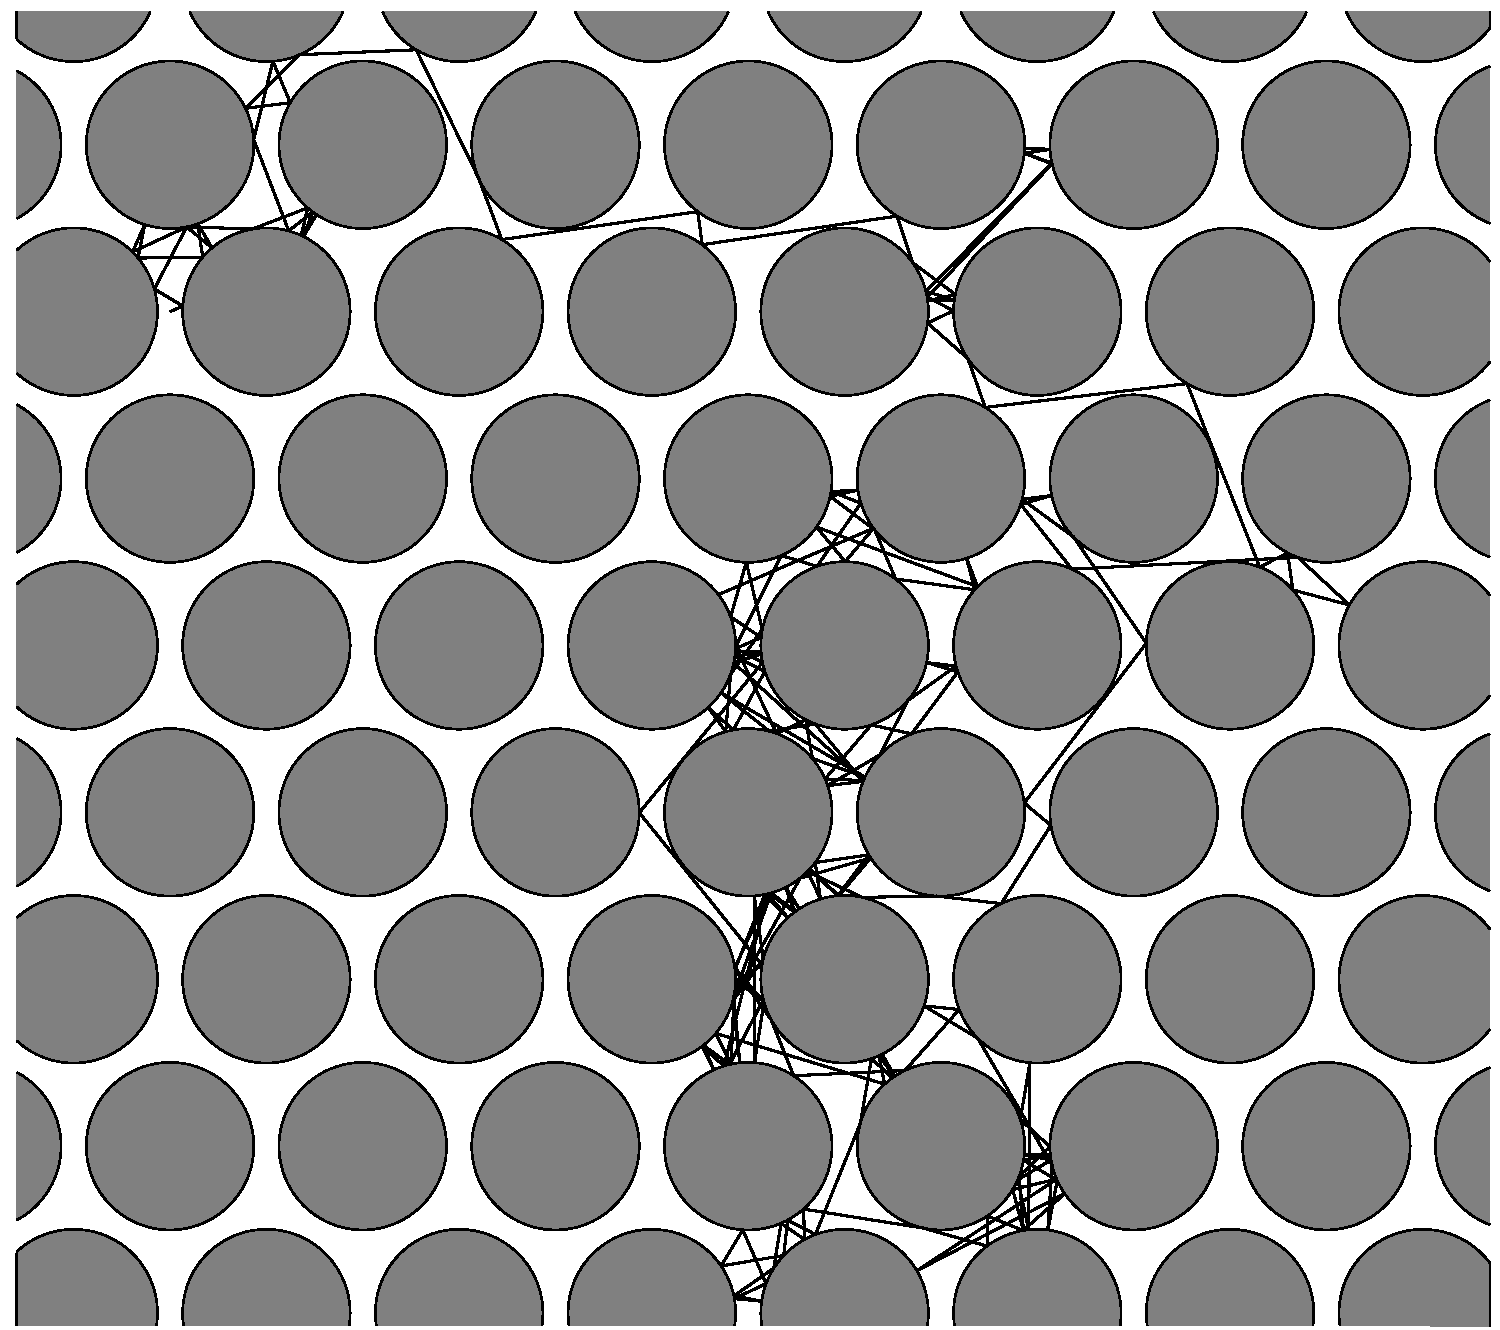
\includegraphics[width=0.45\textwidth]{diffuseChaoticBouncing}
    (b)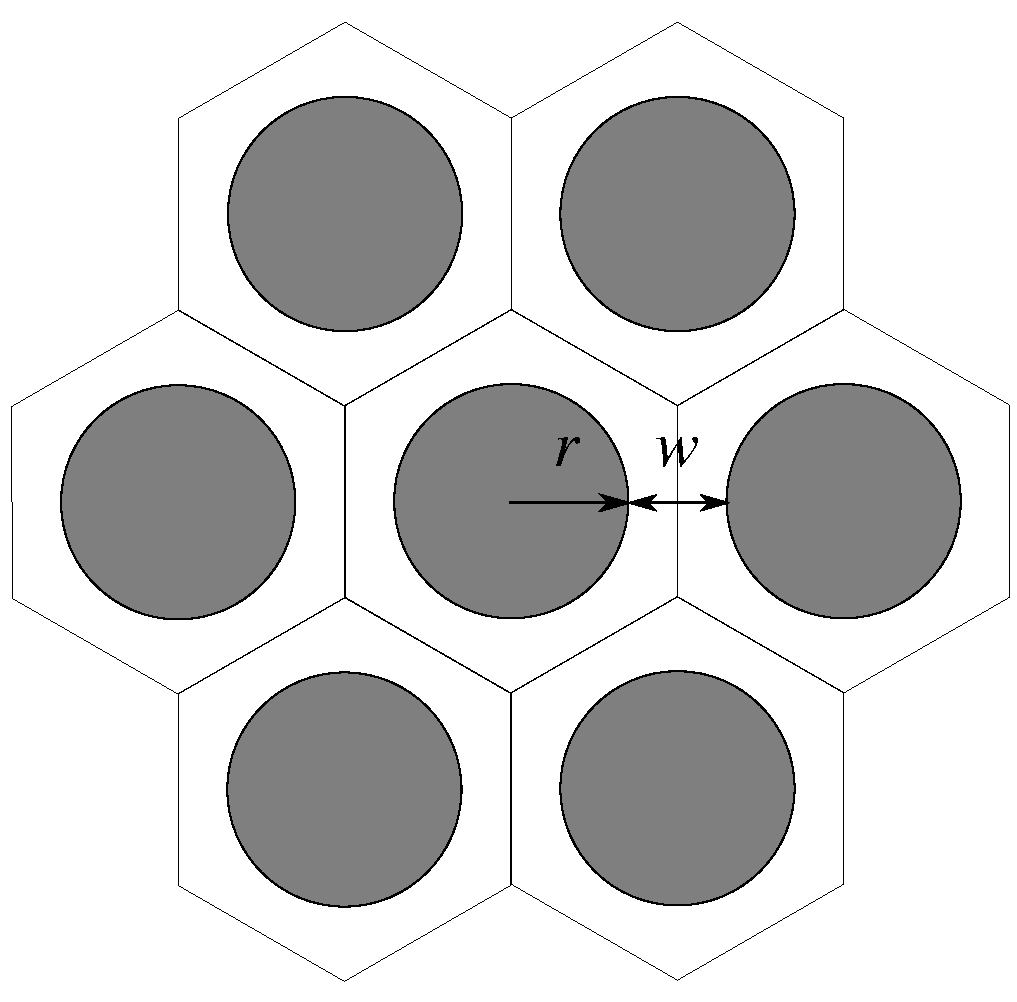
\includegraphics[width=0.45\textwidth]{diffuseLorentzGasParams}
  \end{center}
  \caption[]{\label{fig-chaoticBouncing}
  Motion in the Lorentz gas system. (a)  The chaotic trajectory of a
  ``gas'' particle bouncing in the array of disks  arranged in a
  hexagonal lattice pattern. The distance between disks are close  enough
  such that the particle has no infinite free flight (finite horizon).
  (b) A portion of the triangular Lorentz gas    system. The ratio of
  distance $w$ between the nearest pair of disks to the    disk radius
  $r$ determines the dynamical properties in the system.
  }
\end{figure}


\bigskip
=========== TO REUSE ========

    \PC{the text from Cvitanovi\'c, Gaspard and Schreiber\rf{CGS92}}
In the periodic Lorentz gas\rf{Lorentz1905}
a point particle reflects elastically off
a periodic array of reflecting disks in a plane.
The system can
be thought of as an unfolding of the Sinai billiard\rf{Sinai70}.
The standard diffusion constant can be defined if the particle has a bounded
free path between any two successive bounces.
An example is a triangular array with sufficiently small
inter-disk spacing.
Unfortunately, as we shall see,
the same mechanism that guarantees a finite horizon
also leads to rather awkward pruning of periodic orbits.

    \PC{edits based Cvitanovi\'c,  Eckmann,and Gaspard\rf{LorentzDiff}}
In \refrefs{art91,LorentzDiff,CGS92,Artuso94,CBdiffusion}  an explicit
connection between the global diffusion and the dynamics restricted to
an elementary cell.
Our method applies to any  hyperbolic dynamical system that is
a periodic tiling $\hM=\bigcup_{ \hn \in T} M_{
\hn}$
of the dynamical phase space $\hM$ by {\sl translates}
$M_{\hn}$
of an {\sl elementary cell} $M$, with $T$ the abelian group of lattice
translations.
Furthermore, each elementary cell may be built from a
{\sl fundamental domain}
$\tM$
by the action of a discrete (not necessarily Abelian) group $G$.

                                                            \toCB
Generalization to continuous time\rf{bowen,pexp} amounts to the replacement
%$ z\,=\,e^{-s} $,
$ z^{\period{p}} \rightarrow e^{-s \period{p}} $,
where $\period{p}$ is now the (not necessarily integer)
%{\sl time-}
period of the prime cycle $p$:
$$
Z(\beta,s)\,=\,\prod_{p\in\PP} \exp \left( - {
 \sum_{r=1}^\infty {1 \over r}
 { e^{(\beta \cdot \hn_p- s \period{p}) r } % z^{n_p r}
 \over { | \det \left( {\bf 1}-{\bf J}_p^{r} \right) | } }
 } \right)
\,\, .
%Eq.~(14)
$$


 As we are concerned with the long time behavior,
 this problem can be circumvented
 by replacing $ \hf^t(\tx{\tpk}) $ by the mean
 drift in the $t \rightarrow \infty$ limit.
 $ \hf^t(\tx{\tpk}) $ is a translation in $\hM$ for each
 complete cycle $p$ in $M$, so we replace
 \bea
 \hf^t(\tx{\tpk}) - \tx{\tpk}
 \,\Longrightarrow \,
 &&
 { { \hf^{m_p t}(\tx{\tpk}) - \tx{\tpk} }
 % \over         m_p
 }
    % \,\equiv \, r {\tilde n}_{\tp} (\tx{\tpk})
 \continue
t &=& r \period{\tilde{p}}, \quad m_p = \period{p}/\period{\tilde{p}} \quad \tx \in \tp \,\, ,
 \eea
 in Eq.~(240).
 The magnitude of ${\tilde n}_{\tp}(\tx{\tpk})$, the mean
 global drift per one traversal of the fundamental cycle $\tp$, is
 independent of the starting point, but its direction is not; the
 reason is that each fundamental domain cycle corresponds to a set of
 trajectories in $\hM$.
 The ${1 \over {|G|}} \sum$ average in
 Eq.~(240) then generates all distinct global drift
 directions, so we can again replace the
 sum over cycle points by the factor $\period{\tilde{p}}$, and obtain the
 $Z$ function Eq.~(14) for the $\alpha $ irreducible subspace
 $$
 Z(\beta,s)_\alpha\,=\,\prod_{\tp \in \t{\cal{P}} } \exp
 % \left( -
  % \sum_{r=1}^\infty {1 \over r}
 % {{
  % \chi_\alpha(h^r_{\tp})
  % }
 % \over
 % { | \det \left( \bf{1}-\t{\bf J}_{\tp}^{r} \right) | }
 % }
 % e^{ ( \beta \cdot {\tilde n}_{\tp} - s \period{\tilde{p}}) r}
  % \right)
 \,\, .
 Eq.~(24)
 $$
 $\hn_{\period{\tilde{p}}}(\tx_k)$
%{\tt NOnsense...}
 The leading eigenvalue of the
unsymmetrized
 operator Eq.~(8) is
 the leading eigenvalue of the symmetric subspace for which
 $\chi_\alpha(g)=1$ for all $g \in G$.




Machta and Zwanzig\rf{MacZwa83} have given numerical results
for the diffusion constant in Lorentz gases,  as well as
estimates based on a random walk approximation. We shall follow
their notation and fix the radius of the disks to 1,
assume unit particle speed, and
denote the spacing between the disks by $w$ (see fig.~1).
The horizon is finite for $w < 4/\sqrt{3}-2 = 0.3094\dots$.
